\subsection{The \codesnip{soundecology} R Package}
The \codesnip{soundecology} R package was developed by Luis Villanueva. This package contains algorithms for calculating the major indices, along with some extra abilities. Most importantly, the \codesnip{soundecology} package includes parameters for indices to split files up into smaller pieces for processing, helping to solve the problems outlined in the Benchmarking section. Obviously, each algorithm outputs the index value, however each also outputs specific values, value lists, and matrices that are also used heavily in this service for creating the visualizations.

\subsubsection{ACI Algorithm}
The ACI algorithm outputs more useful information than most of the other algorithms. In addition to the base ACI value, it outpus an ACI value by minute, which is a bit better representation of the ACI, especially for longer files. It also outputs a list of ACI values for each bin, which all sum up to the total ACI value. This list is useful for creating the line graphs included in this service. More information on the ACI index can be found in the Overview of Indices section.

\subsubsection{NDSI Algorithm}
The core NDSI algorithm that comes with the soundecology package outputs everything needed for this service, so no changes are needed. Those outputs include the NDSI values for both channels, as well as the biophony and anthrophony for both channels. These values are used for the visualizations, expanded upon in the Data Visualizations Research section.

\subsubsection{ADI and AEI Algorithm}
As ADI and AEI are closely related, their outputs are mostly the same, just tailored to the respective index. Along with the actual ADI or AEI value, the algorithms also output the ADI or AEI value for each band range, which is not included natively for AEI in the R package, and is included in the Proposed Changes section. These values include the ADI or AEI value at each frequency range, which can be specified by the user when creating jobs. Using these outputs, the ADI and AEI charts are able to be made.

\subsubsection{Bioacoustic Index Algorithm}
For the Bioacoustic index, the outputs for this service also include the left and right values, as well as the left and right normalized values for each frequency range. This is different than the base \codesnip{soundecology} package, and these changes are explained in the Proposed Changes section. For more information on how the Bioacoustic index is calculated, see the Overview of Indices section.

\subsubsection{R Package Values}

These tables show the default parameter values for each of the Soundecology algorithms.\par

% Table formatting
\newcommand{\parameter}{2.5cm}
\newcommand{\default}{3.5cm}

\paragraph{Acoustic Complexity Index (ACI)} \mbox{}\\[\longtableheaderspace]
\begingroup
\renewcommand{\arraystretch}{\cellpaddingvertical}
\begin{longtable}{| m{\parameter} | m{\default} |}
  \hline
  \tablehead{Parameter}
  & \tablehead{Default}
  \\ \hline

  minFreq
  & 0 Hz
  \\ \hline

  maxFreq
  & Max frequency for file in Hz
  \\ \hline

  j
  & 5 seconds
  \\ \hline

  fftW
  & 512
  \\ \hline
\end{longtable}
\endgroup


\paragraph{Normalized Difference Soundscape Index (NDSI)} \mbox{}\\[\longtableheaderspace]
\begingroup
\renewcommand{\arraystretch}{\cellpaddingvertical}
\begin{longtable}{| m{\parameter} | m{\default} |}
  \hline
  \tablehead{Parameter}
  & \tablehead{Default}
  \\ \hline

  fftW
  & 1024
  \\ \hline

  anthroMin
  & 1000 Hz
  \\ \hline

  anthroMax
  & 2000 Hz
  \\ \hline

  bioMin
  & 2000 Hz
  \\ \hline
  
  bioMax
  & 11000 Hz
  \\ \hline
\end{longtable}
\endgroup


\paragraph{Acoustic Diversity Index (ADI)} \mbox{}\\[\longtableheaderspace]
\begingroup
\renewcommand{\arraystretch}{\cellpaddingvertical}
\begin{longtable}{| m{\parameter} | m{\default} |}
  \hline
  \tablehead{Parameter}
  & \tablehead{Default}
  \\ \hline

  maxFreq
  & 10000 Hz
  \\ \hline

  dbThreshold
  & -50 dBFS
  \\ \hline

  freqStep
  & 1000
  \\ \hline

  shannon
  & true
  \\ \hline
\end{longtable}
\endgroup


\paragraph{Bioacoustic Index} \mbox{}\\[\longtableheaderspace]
\begingroup
\renewcommand{\arraystretch}{\cellpaddingvertical}
\begin{longtable}{| m{\parameter} | m{\default} |}
  \hline
  \tablehead{Parameter}
  & \tablehead{Default}
  \\ \hline

  minFreq
  & 2000 Hz
  \\ \hline

  maxFreq
  & 8000 Hz
  \\ \hline

  fftW
  & 512
  \\ \hline
\end{longtable}
\endgroup


\paragraph{Acoustic Evenness Index} \mbox{}\\[\longtableheaderspace]
\begingroup
\renewcommand{\arraystretch}{\cellpaddingvertical}
\begin{longtable}{| m{\parameter} | m{\default} |}
  \hline
  \tablehead{Parameter}
  & \tablehead{Default}
  \\ \hline

  maxFreq
  & 10000 Hz
  \\ \hline

  dbThreshold
  & -50 dBFS
  \\ \hline

  freqStep
  & 1000
  \\ \hline
\end{longtable}
\endgroup

\subsubsection{Soundecology Package Dependencies}
The core soundecology package does not handle wav file conversion to Wav object that is needed for use in the algorithms. This is handled by a package named tuneR, which takes in audio files and converts them to R objects compatible with the R algorithms in soundecology. This is the only package that is of any note, as it will require its own set of instructions during our processing of the user\textquotesingle s files. The script for converting a user file into a Wav object is the following

\begin{javascriptcode}
  tdir <- getwd()
  tfile <- file.path(tdir, "SoundFileName.wav")
  newWobj <- readWave(tfile)
  result <- ndsi(newWobj)
\end{javascriptcode}

In order for this to work, the current working directory must be set to where the user\textquotesingle s files are located, and the SoundFileName must match the user\textquotesingle s as well. Luckily soundecology \textit{does} have a method, multiple_sounds, for going through all files in a subdirectory, and handles this natively. However multiple_sounds only goes through a directory, not for single file use.

\subsubsection{Proposed Changes}
For use in our service, this R package needs to be modified. Namely, the Bioacoustic index and AEI outputs need to be more detailed. For Bioacoustic, the bioacoustic values for both the left and right channels need to be output, along with the normalized left and right channel values. These values are in turn used in our visualizations to create the area graphs shown in the Data Visualizations Research section. As for AEI, it just needs to be changed to match that of the ADI. For whatever reason, the core package outputs only the AEI values for the left and right channel, and did not output the left and right band values and left and right band ranges. These are also used in the AEI and ADI visualizations.\par
Another proposed change that is talked about a bit in the Benchmarking section, is that of file size constraints. Currently, certain indices are not able to be computed on long files due to hardware limitations even on high end systems. These memory issues are the result of matrices being created in indices like ACI. From reviewing the code, these matrices are being used as intermediary values used in the calculation of lists of \textit{more} intermediary values. These matrices are in fact output to the user, however the usefulness of them is up for debate. Proposed changes to circumvent these issues include possibly removing these matrices, or adding a file splicing feature. Files that are over a certain length would need to be split into equal length parts, and the index would be calculated on each. From there, the overall index value could be calculated either in R or in the client.

\subsubsection{Vectorization}
One of the main reasons for this project was to increase the efficiency of our sponsor's work flow. We realized that ACI was one of the most intensive indices to run so it made sense to look at it first. That being said, one of the biggest problems with the original code is its use of for loops. R is notoriously slow at looping with the only solution being to vectorize the functions you write. To do this we took algorithms being run inside of a for loop and made them in to seperate functions. Once sectioned off these functions could be appropriated to take in vectors and output vectors. This also involved adjusting some of the code after functions to work strictly with vectors. This led to a speed up close to 60\% on an 18 second sound file.

\begin{center}
	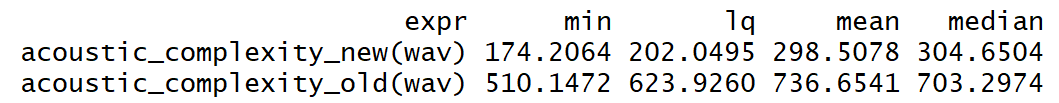
\includegraphics[width=0.85\textwidth]{ACIBenchmark} \\[12pt]
\end{center}

\subsubsection{Memory Challenges}
One of the major challenges that we encountered with the processing of sound files was the massive amounts of RAM needed. We identified the problem to be a third party function called \codesnip{spectro}. Out of the 152MB used to process the 18 second sound file 146MB was used by two instances of \codesnip{spectro}.\par
The first approach was to look for alternatives, but the basic functionality of \codesnip{spectro} made it so that all substitutes also used massive amounts of memories. Once we dove into how \codesnip{spectro} worked we realized that it was used to make a matrix that represented the intensity of the sound file at every frequency over time. By its very nature the function was going to need a large amount of memory.\par
The second solution was to split the files on the window length and run \codesnip{spectro} on smaller chunks. This would increase the run-time of the analysis slightly but reduced the RAM used on an hour long file from 9GB to just under 2GB. The issue with this is that slicing the sound file produced slightly different numbers than the original function. Once we looked into the reason it was found that slicing the files made it so that the \codesnip{spectro} function took its measurements at different points. We decided that this would be a problem better solved by someone who had a deeper understanding of the mathematics behind the ACI index.\par
Our final solution was to just limit one job at a time for our application and to require a minimum number of Gig's in order to run our program. While this solution was less than desired we believe that this is something that is not crucial to the product working. That being said this would be an excellent point of improvement for future groups who may be more focused on the research side of this application.\par
\subsubsection{Minor Improvements}
Some small changes were made in order to try and improve the memory usage of the ACI index algorithm. The matrix of intensity changes, used to calculate ACI values, was replaced with on-going calculations. An option was added to include the matrix if desired. With the matrix disabled the memory cost for storing the output decreased from 80KB to 15KB. This improvement is expected to drastically help reduce the size of our database storage needs.